% KU Leuven latex presentation template
%
% © 2012 Michael Hofmann
%
% This work is licensed under the Creative Commons Attribution 3.0 Unported License.
% To view a copy of this license, visit
% http://creativecommons.org/licenses/by/3.0/ or send a letter to Creative
% Commons, 444 Castro Street, Suite 900, Mountain View, California, 94041, USA.

\documentclass[t,12pt,english
\ifx\beamermode\undefined\else,\beamermode\fi
]{beamer}
%\setbeameroption{show notes}
%\setbeameroption{show only notes}

\usepackage[utf8]{inputenc}
\usepackage[T1]{fontenc}
\usepackage{amsmath}
\usepackage[nohyperlinks]{acronym}
\usepackage{babel,lmodern,graphicx,mathptmx,xspace,wasysym,microtype,booktabs,tabularx,relsize,textcomp,longtable,lipsum,colortbl,eurosym,url,multicol,etoolbox,multimedia,pdfpages,fixltx2e,ifluatex,epstopdf}
\usepackage[olditem,oldenum]{paralist}
\usepackage[babel=true]{csquotes}
\usepackage[thinqspace,amssymb,textstyle]{SIunits}
\usepackage[textsize=tiny]{todonotes}
\usepackage[symbol]{footmisc}
\usepackage[notquote]{hanging}
\usepackage[normalem]{ulem}
\usepackage{comment}
\usepackage{media9}
%\usepackage{lua-visual-debug}

\pdfstringdefDisableCommands{\renewcommand{\sout}{}}
\graphicspath{{Images/}}
% Fix sort order in case the same file exists with multiple extensions
\DeclareGraphicsExtensions{.pdf,.png,.jpeg,.jpg,.eps}
\frenchspacing

\input{templates/definitions.tex}

%% From pandoc default template
% End pandoc

\mode<presentation>

%\hypersetup{pdfpagemode=FullScreen}

\definecolor{kuldefault}{HTML}{00407a}
\definecolor{kulbright}{HTML}{52bdec}
\definecolor{kulleft}{HTML}{1d8db0}
\definecolor{kulright}{HTML}{116e8a}

\definecolor{kulyellow}{HTML}{BC8F00}
\definecolor{kulorange}{HTML}{BC6E00}
\definecolor{kulgreen}{HTML}{007F4F}
\definecolor{kulred}{HTML}{FF4422}

\setbeamercolor{structure}{fg=kulbright}
\setbeamercolor{title}{fg=white}
\setbeamercolor{footline}{parent=title}
\setbeamercolor{normal text}{fg=kuldefault}
\setbeamercolor{item}{parent=normal text}
\setbeamercolor{section in toc}{parent=normal text}
\setbeamerfont{title}{size=\Large}
\setbeamerfont{tiny structure}{series=\bfseries}
\setbeamerfont{caption}{}

\setbeamersize{text margin left=0.8cm}
\setbeamersize{text margin right=0.8cm}
\setbeamersize{sidebar width left=0cm}

\setbeamertemplate{navigation symbols}{}
\setbeamertemplate{itemize item}{\footnotesize\raise1pt\hbox{\textbullet}}
\setbeamertemplate{itemize subitem}{--}
\setbeamertemplate{itemize subsubitem}{\tiny\raise1.5pt\hbox{\textbullet}}

\setlength\leftmargini{1em}
\setlength\leftmarginii{1em}
\setlength\leftmarginiii{1em}




\defbeamertemplate{background canvas}{title}
{%
    \pgfdeclarehorizontalshading{bgshading}{8.70cm}{color(0cm)=(kulleft); color(\the\paperwidth)=(kulright)}%
    \vbox to 8.70cm{%
        \pgfuseshading{bgshading}\hspace*{-1.6cm}%
    }%
    \hskip-\paperwidth%
    \hskip1.6cm%
    \vbox to \paperheight{%
        \vskip0.1cm\hskip0.1cm\includegraphics[width=2.83cm]{templates/kuleuven}%
        \vskip0.99cm\hskip0.76cm\includegraphics[width=2.84cm]{templates/key}%
        \vskip-0.57cm\hskip11.61cm\includegraphics[width=0.58cm]{templates/sedes}\hspace*{-1cm}%
        \vfill
    }%
}

\defbeamertemplate{background canvas}{grid}
{%
    \begin{tikzpicture}[remember picture,overlay,every node/.style={anchor=center}]
        \foreach \d in {0,...,20} {
            \draw[gray] (\d,0) -- (\d,-20);
            \draw[gray] (0,-\d) -- (20,-\d);
            \draw[lightgray] (\d+0.5,0) -- (\d+0.5,-20);
            \draw[lightgray] (0,-\d-0.5) -- (20,-\d-0.5);
            \node[anchor=north,red,font=\tiny] at (\d,0) {\d};
            \node[anchor=west,red,font=\tiny] at (0,-\d) {\d};
        }
    \end{tikzpicture}
}

\defbeamertemplate{background canvas}{plain}{}

\defbeamertemplate{footline}{large}
{%
    \pgfdeclarehorizontalshading{bgshading}{0.62cm}{color(0cm)=(kulleft); color(\the\paperwidth)=(kulright)}%
    \vskip.3cm% make room for the logo
    \parbox[t][0.62cm]{\paperwidth}{\pgfuseshading{bgshading}}\par%
    \vskip-0.62cm%
    \begin{beamercolorbox}[ht=0.37cm,dp=0.25cm,center]{page number in head/foot}%
    \insertframenumber%
    \end{beamercolorbox}%
    \vskip-0.92cm%
    \parbox[t][0.92cm]{\paperwidth}{\hskip10.33cm\includegraphics[width=2.10cm]{templates/kuleuven}}\par%
}

\defbeamertemplate{footline}{nopagenumber}
{%
    \pgfdeclarehorizontalshading{bgshading}{0.62cm}{color(0cm)=(kulleft); color(\the\paperwidth)=(kulright)}%
    \vskip.3cm% make room for the logo
    \parbox[t][0.62cm]{\paperwidth}{\pgfuseshading{bgshading}}\par%
    \vskip-0.62cm%
    \begin{beamercolorbox}[ht=0.37cm,dp=0.25cm,center,ignorebg]{page number in head/foot}%
    %
    \end{beamercolorbox}%
    \vskip-0.92cm%
    \parbox[t][0.92cm]{\paperwidth}{\hskip10.33cm\includegraphics[width=2.10cm]{templates/kuleuven}}\par%
}

\defbeamertemplate{footline}{small}
{%
    \vskip.3cm% make room for the logo
    \begin{beamercolorbox}[ht=0.5cm,dp=0.5cm,center,ignorebg]{normal text}%
    \mdseries\insertframenumber%
    \end{beamercolorbox}%
}

\setbeamertemplate{footline}[large]

\setbeamertemplate{frametitle}
{%
    \nointerlineskip%
    \vskip.28cm%
    {\usebeamercolor[fg]{framesubtitle}\usebeamerfont{framesubtitle}\insertsupertitle\strut\par}%
    \vskip-.2cm%
    {\usebeamercolor[fg]{frametitle}\usebeamerfont{frametitle}\insertframetitle\strut\par}%
    \vskip-.3cm%
}

\setbeamertemplate{title page}
{
    \vbox{}%
    \vskip2.8cm%
    \vbox to 6.5cm{%
        \hskip2.8cm%
        \begin{minipage}{7.9cm}
            \begin{beamercolorbox}{title}
                \usebeamerfont{title}%
                \inserttitle\par%
                \ifx\insertsubtitle\undefined%
                \else%
                    \vskip0.25em%
                    {\usebeamerfont{subtitle}\usebeamercolor[fg]{subtitle}\insertsubtitle\par}%
                \fi%
            \end{beamercolorbox}%
            \vskip1em\par
            \begin{beamercolorbox}{author}
                \usebeamerfont{author}\usebeamercolor[fg]{subtitle}%
                \insertauthor
            \end{beamercolorbox}
            \begin{beamercolorbox}{institute}
                \usebeamerfont{institute}\usebeamercolor[fg]{subtitle}%
                \insertinstitute
                \end{beamercolorbox}
            \begin{beamercolorbox}{date}
                \usebeamerfont{date}\usebeamercolor[fg]{subtitle}%
                \insertdate
            \end{beamercolorbox}%
        \end{minipage}%
        \vfill
    }
}

\mode<all>

\newcommand{\inlinesound}[2]{\movie[inlinesound,encoding=Signed,samplingrate=44100]{#1}{#2}}

% disable for now as otherwise all commands that go between frames generated by
% the filter will result in duplicate toc lines
\renewcommand{\addcontentsline}[3]{}

\newcommand{\largefooter}{\setbeamertemplate{footline}[large]}
\newcommand{\emptyfooter}{\setbeamertemplate{footline}[nopagenumber]}
\newcommand{\smallfooter}{\setbeamertemplate{footline}[small]}

\newcommand{\sectiontoc}{\AtBeginSection[]{{
    \nosupertitle
    \emptyfooter
    \begin{frame}[noframenumbering]{Outline}
                \tableofcontents[currentsection]
            \end{frame}
    \largefooter
}}}

\newcommand{\subsectiontoc}{\AtBeginSubsection[]{{
    \nosupertitle
    \emptyfooter
    \begin{frame}[noframenumbering]{Outline}
                \tableofcontents[currentsection,currentsubsection]
           \end{frame}
    \largefooter
}}}

\newcommand{\notoc}{\AtBeginSection[]{}\AtBeginSubsection[]{}}

\newcommand{\nosupertitle}{\renewcommand{\insertsupertitle}{}}
\newcommand{\sectiontitle}{\renewcommand{\insertsupertitle}{\insertsectionhead}}
\newcommand{\subsectiontitle}{\renewcommand{\insertsupertitle}{\insertsectionhead\ifx\insertsubsectionhead\empty\else{} -- \insertsubsectionhead\fi}}

% animations do not work atm as figures are set on independent frames
\newcommand{\slidefig}[2]{\usebackgroundtemplate{\parbox[c][\paperheight][c]{\paperwidth}{\centering\includegraphics#1[height=\paperheight,width=\paperwidth,keepaspectratio]{#2}}}\begin{frame}[plain]\end{frame}\usedefaultcanvas}

\newcommand{\usedefaultcanvas}{\setbeamertemplate{background canvas}[\defaultcanvas]}
\newcommand{\gridcanvas}{\renewcommand{\defaultcanvas}{grid}\usedefaultcanvas}
\newcommand{\plaincanvas}{\renewcommand{\defaultcanvas}{plain}\usedefaultcanvas}

\newcommand{\insertsupertitle}{}






\newcommand{\defaultcanvas}{plain}


% Defining a new coordinate system for the page:
%
% ----------------
% |(0,1)    (1,1)|
% |              |
% |(0,0)    (1,0)|
% ----------------
\makeatletter
\def\parsecomma#1,#2\endparsecomma{\def\page@x{#1}\def\page@y{#2}}
\tikzdeclarecoordinatesystem{page}{
    \parsecomma#1\endparsecomma
    \pgfpointanchor{current page}{north east}
    % Save the upper right corner
    \pgf@xc=\pgf@x%
    \pgf@yc=\pgf@y%
    % save the lower left corner
    \pgfpointanchor{current page}{south west}
    \pgf@xb=\pgf@x%
    \pgf@yb=\pgf@y%
    % Transform to the correct placement
    \pgfmathparse{(\pgf@xc-\pgf@xb)*\page@x+(\pgf@xb)}
    \expandafter\pgf@x\expandafter=\pgfmathresult pt
    \pgfmathparse{(\pgf@yc-\pgf@yb)*\page@y+(\pgf@yb)}
    \expandafter\pgf@y\expandafter=\pgfmathresult pt
}
\makeatother

% Example:
%\begin{tikzpicture}[remember picture,overlay,every node/.style={anchor=center}]
%  \node at (page cs:0.5,0.3) {0.5,0.3};
%  \node at (page cs:0,0) {0,0};
%  \draw(page cs:0,0) -- (page cs:1,1);
%  \draw[thick,red] (page cs:0,0) rectangle (page cs:1,1);
%  \draw[thick,green] (page cs:0.2,0.2) rectangle (page cs:0.8,0.8);
%\end{tikzpicture}

\setcounter{secnumdepth}{0}

\title{\large HD-PULSE: a new open platform for 3D ultrasound imaging}

\author{\\ \href{vangjush.komini@uzleuven.be}{\textbf{\textit{Vangjush Komini}}}
}



\institute{\href{www.kul.be}{KU Leuven}}
\date{\vspace{.10cm}Novermber $16^{th}$ 2015}

\begin{document}

\setbeamertemplate{background canvas}[title]

\begin{frame}[plain,noframenumbering]
    \titlepage
\end{frame}

\usedefaultcanvas


\emptyfooter
\begin{frame}[noframenumbering]{Outline}
        \tableofcontents
    \end{frame}
\largefooter



\section{System specification}\label{first-section}


\begin{frame}{Functional requirements}

\begin{figure}[!htb]
\minipage{0.5\textwidth}
\begin{block}{\footnotesize{}}\tiny{}
\begin{enumerate} 
\vspace{0.05cm}
     \item \tiny{\textbf{\textit{Fast computation, high throughput}}} \tiny{hardware parallelism}
     \item \tiny{\textbf{\textit{Time to Market small}}} \tiny{highly flexible and prototypable} 
     \item \tiny{\textbf{\textit{Cost}}} \tiny{NRE nonrecurring engineering expense of custom}
     \item \tiny{\textbf{\textit{Reliability}}} \tiny{"hard" implementation in circuit}
     \item \tiny{\textbf{\textit{Long-Term Maintenance}}} \tiny{field upgradable, no time for redesigning as ASIC}
\end{enumerate}
\end{block}
\endminipage
\minipage{0.8\textwidth}
\endminipage
\end{figure}

\end{frame}

\begin{frame}{Functional requirements}

\begin{figure}[!htb]
\minipage{0.5\textwidth}
\begin{block}{\footnotesize{}}\tiny{}
\begin{enumerate} 
\vspace{0.05cm}
     \item \tiny{\textbf{\textit{Fast computation, high throughput}}} \tiny{hardware parallelism}
     \item \tiny{\textbf{\textit{Time to Market small}}} \tiny{highly flexible and prototypable} 
     \item \tiny{\textbf{\textit{Cost}}} \tiny{NRE nonrecurring engineering expense of custom}
     \item \tiny{\textbf{\textit{Reliability}}} \tiny{"hard" implementation in circuit}
     \item \tiny{\textbf{\textit{Long-Term Maintenance}}} \tiny{field upgradable, no time for redesigning as ASIC}
\end{enumerate}
\end{block}

\includegraphics[width=.75\textwidth]{1_1.png}
\endminipage
\minipage{0.5\textwidth}
\centering
\includegraphics[width=.65\textwidth]{3.png}
\endminipage
\end{figure}

\end{frame}

\emptyfooter
\begin{frame}{}
\begin{figure}[!htb]
\includegraphics[width=.91\textwidth]{6.png}
\end{figure}
\largefooter
\end{frame}

\begin{frame}{Mileston}

\begin{block}{\footnotesize{High data rate acquisition is the \textbf{highlight} of the system}}\tiny{}
\begin{enumerate} 
\vspace{0.05cm}
     \item \tiny{\textbf{\textit{Probe to FPGA}} } 
     \item \tiny{FPGA to HOST}
\end{enumerate}
\end{block}

\begin{figure}[!htb]
\minipage{0.5\textwidth}
\includegraphics[width=.81\textwidth]{2.png}
\caption{\tiny{Probe Interface}}
\endminipage
\minipage{0.5\textwidth}
\centering
\includegraphics[width=1\textwidth]{4.png}
\caption{\tiny{FPGA to HOST} }
\endminipage
\end{figure}

\end{frame}

\subsection{Outline of the FPGA}
\begin{frame}{FlexRIO}

High data rate acquisition is the \textbf{highlight} of the system

\begin{figure}[!htb]
\includegraphics[width=.51\textwidth]{5.png}
\caption{\tiny{FlexRIO with module}}
\end{figure}

\end{frame}

\emptyfooter
\begin{frame}{}
\begin{figure}[!htb]
\includegraphics[width=.91\textwidth]{2_1.png}
\end{figure}
\largefooter
\end{frame}


\subsection{Multiplexer}
\begin{frame}{DSL32M}



\begin{figure}[!htb]
\minipage{0.5\textwidth}

\begin{block}{\footnotesize{Multiplexer module}}\footnotesize{}
\begin{enumerate} 
\vspace{0.05cm}
     \item \footnotesize{32 channels}
     \item \footnotesize{Independent high voltages}
     \item \footnotesize{Bi-directional switches}
     \item \footnotesize{SPI interfacing}
     \item \footnotesize{Stackable with daisy chain}
\end{enumerate}
\end{block}

\endminipage
\minipage{0.5\textwidth}
\centering
\includegraphics[width=.85\textwidth]{9.png}
\caption{\tiny{DSL32M module}}
\endminipage
\end{figure}

\end{frame}

\emptyfooter
\begin{frame}{}
\begin{figure}[!htb]
\includegraphics[width=.91\textwidth]{2_2.png}
\end{figure}
\largefooter
\end{frame}


\subsection{Pulser}
\begin{frame}{DSL32T}



\begin{figure}[!htb]
\minipage{0.5\textwidth}

\begin{block}{\footnotesize{Pulser}}\footnotesize{}
\begin{enumerate} 
\vspace{0.05cm}
     \item \footnotesize{32 channels}
     \item \footnotesize{Independent high voltages}
     \item \footnotesize{Programmable sequence}
     \item \footnotesize{3-level output}
     \item \footnotesize{External HV power}
     \item \footnotesize{Power to muxer}
     \item \footnotesize{SPI interfacing}
\end{enumerate}
\end{block}

\endminipage
\minipage{0.5\textwidth}
\centering
\includegraphics[width=.85\textwidth]{11.png}
\caption{\tiny{DSL32T module}}
\endminipage
\end{figure}

\end{frame}




\emptyfooter
\begin{frame}{}
\begin{figure}[!htb]
\includegraphics[width=.91\textwidth]{2_3.png}
\end{figure}
\largefooter
\end{frame}


\subsection{Module}
\begin{frame}{DSL32R}

\begin{figure}[!htb]
\minipage{0.5\textwidth}
\begin{block}{\footnotesize{Front end pulser}}\footnotesize{}
\begin{enumerate} 
\vspace{0.01cm}
     \item \footnotesize{32 channels}
     \item \footnotesize{LN pre-A}
     \item \footnotesize{Tx/Rx protection}
     \item \footnotesize{Power supply to muxer}
     \item \footnotesize{External clock to digitizer}
     \item \footnotesize{SPI interface}
\end{enumerate}
\end{block}

\endminipage
\minipage{0.5\textwidth}
\centering
\includegraphics[width=1\textwidth]{7.png}
\caption{\tiny{DSL32R module}}
\endminipage
\end{figure}

\end{frame}



\emptyfooter
\begin{frame}{}
\begin{figure}[!htb]
\includegraphics[width=.91\textwidth]{2_4.png}
\end{figure}
\largefooter
\end{frame}

\subsection{ADC}
\begin{frame}{NI5752}



\begin{figure}[!htb]
\minipage{0.5\textwidth}

\begin{block}{\footnotesize{Receiver}}\footnotesize{}
\begin{enumerate} 
\vspace{0.05cm}
     \item \footnotesize{32 channels digitizer}
     \item \footnotesize{Digitally controlled swept gain}
     \item \footnotesize{Programmable filters}
     \item \footnotesize{SPI interfacing}
     \item \footnotesize{External clock}
     \item \footnotesize{Digital control to the adapter}
\end{enumerate}
\end{block}

\endminipage
\minipage{0.5\textwidth}
\centering
\includegraphics[width=.95\textwidth]{8.png}
\caption{\tiny{NI5752 module}}
\endminipage
\end{figure}
\end{frame}

\section{System operation}\label{second-section}


\emptyfooter
\begin{frame}{}
\centering
\vspace{3cm}
\Huge System operation 



\end{frame}
\largefooter





\emptyfooter
\begin{frame}{}
\begin{figure}[!htb]
\centering
\includegraphics[width=1.1\textwidth]{12.png}
\end{figure}
\end{frame}
\largefooter

\begin{frame}{Acquisition modalities}

\begin{block}{\footnotesize{DSLFITfocusStream}}\footnotesize{}
\begin{enumerate} 
\vspace{0.05cm}
     \item \footnotesize{Beam-forming in FPGA}
     \item \footnotesize{Data streamed to host via DRAM buffer}
     \item \footnotesize{Linear, Sector scans with A, B, C scans}
\end{enumerate}
\end{block}

\begin{block}{\footnotesize{DSLFITacquire}}\footnotesize{}
\begin{enumerate} 
\vspace{0.05cm}
     \item \footnotesize{Parallel channel acquisition and transfer}
     \item \footnotesize{Batch mode acquisition}
     \item \footnotesize{FMC, FRD and Linear Acquisition}
\end{enumerate}
\end{block}
\end{frame}

\begin{frame}{SW Framework}

\begin{figure}[!htb]
\minipage{0.5\textwidth}

\begin{block}{\footnotesize{}}\footnotesize{}
\begin{enumerate} 
\vspace{0.05cm}
     \item \footnotesize{Determine the available HW}
     \item \footnotesize{Initialise FPGA of any $DSL32T$}
     \item \footnotesize{Initialise FPGA of any $NIT5752$ }
     \item \footnotesize{Initialise all variables}
     \item \footnotesize{Queued State Machine loop}
     \item \footnotesize{Event Handler for GUI}
     \item \footnotesize{Close FPGA referencse on exit}
\end{enumerate}
\end{block}

\endminipage
\minipage{0.5\textwidth}
\centering
\includegraphics[width=1.1\textwidth]{13.png}
\endminipage
\end{figure}

\end{frame}

\begin{frame}{Configuration}

\begin{figure}[!htb]
\minipage{0.5\textwidth}

\endminipage
\minipage{0.5\textwidth}
\centering
\includegraphics[width=1\textwidth]{14.png}
\endminipage
\end{figure}

\begin{figure}[!htb]
\minipage{0.5\textwidth}
\centering
\includegraphics[width=1\textwidth]{15.png}
\endminipage
\minipage{0.5\textwidth}
\centering
\includegraphics[width=1\textwidth]{16.png}
\endminipage
\end{figure}

\end{frame}

\begin{frame}{User interface}

\begin{figure}[!htb]
\minipage{0.5\textwidth}

\endminipage
\centering
\includegraphics[width=1\textwidth]{17.png}
\end{figure}

\end{frame}

\emptyfooter
\begin{frame}{ }
\centering \textbf{\Large \textit{Thank you for your attention}}
\begin{figure}[!htb]
\includegraphics[width=.6\textwidth]{QA.jpg}
\end{figure}
\largefooter
\end{frame}


\begin{frame}[allowframebreaks]
        \frametitle{References}
        \bibliography{main}
        \bibliographystyle{plain}
\end{frame}


\end{document}
